\chapter{Fundamentação Teórica}
\label{chap:fundamentacao}

Nesse capítulo são apresentados os principais conceitos necessários para entendimento do presente trabalho. Na Seção \ref{sec:dsl} serão apresentados os conceitos sobre \gls{DSL}, tais como: diferenças sobre as linguagens convencionais de programação, vantagens e desafios, ferramentas de construção e por fim será apresentada a justificativa de escolha da ferramenta \gls{MPS} para o desenvolvimento desta proposta.


\section{Linguagens Específicas de Domínio}
\label{sec:dsl}

Para \citeonline{kernelif}, a necessidade de abstrações personalizadas sobre um núcleo funcional originam as linguagens de domínio específicos, \gls{DSL}s. Para \citeonline{spinellis2001notable} \gls{DSL}s são, por definição, parte de um sistema maior e geralmente implementado para uso específico de domínio.

\citeonline{mernik2005and}, afirmam que as \gls{DSL}s fornecem construções sob medida para um domínio específico de aplicativo, fornecendo ganhos substanciais em expressividade e facilidade do uso quando comparado com as \gls{GPL}, o que corresponde em ganhos de produtividade e redução nos custos de manutenção.

No que concerne às questões de comunicação, \citeonline{ghosh2011dsl} descreve que uma \gls{DSL} preenche a lacuna semântica entre usuários de negócio e desenvolvedores, incentivando uma melhor colaboração por meio de vocabulário compartilhado.  

Segundo \citeonline{mernik2005and}, são exemplos de linguagens de domínio específico: HTML, Latex, SQL, Excel, etc. As linguagens possuem domínios de aplicação diferenciados (Figura \ref{fig:exemplosdsl}), e a sua aplicação pode reduzir a expertise necessária de programação para seus usuários .


\begin{figure}[h!]
\centering

\caption{\textmd{Exemplos de DSL amplamente utilizadas}}
\label{fig:exemplosdsl}
\fcolorbox{gray}{white}{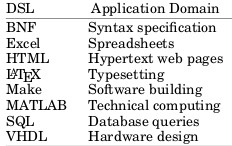
\includegraphics[width=0.4\textwidth]{chapters/fundamentacao/imagens/exemplosdsl.jpg}}

\par\medskip\textbf{Fonte:} \citeonline{mernik2005and}. \par\medskip
\end{figure}


As \gls{DSL}s podem ser classificadas de acordo com a sua implementação, se construídas para serem incorporadas em uma \gls{GPL} elas podem ser consideradas como \gls{DSL}s internas, enquanto as externas são independentes da infraestrutura de uma linguagem de programação existente \cite{dslengineering}.

\citeonline{fowler2005language} define \gls{DSL}s externas e internas como:

\begin{citacao} 
\gls{DSL} externa é aquela que é escrita em uma linguagem separada da linguagem principal da aplicação, \textit{Unix little languages} e arquivos de configuração de \gls{XML} são bons exemplos desse estilo de linguagem. Enquanto as \gls{DSL} internas são limitadas pela sintaxe e estrutura da linguagem base em que são criadas, recursos de linguagem como \textit{closures}, \textit{macros} são exemplos de construção de linguagens internas \cite[s/p, tradução nossa]{fowler2005language}.
\end{citacao}


Nesse contexto, o presente trabalho objetiva a criação de uma \gls{DSL} externa, com sua própria sintaxe e semântica, de modo que seja possível especificar regras do sistema de cotas da rede de ensino pública federal, de maneira independente à linguagem de programação alvo do sistema. 

\subsection{Diferenças sobre linguagens convencionais}
\label{diferencasdsl}

Segundo \citeonline{dslengineering}, o propósito das \gls{DSL} é de atender a um domínio específico, são construídas para resolver uma classe específica de problemas. De outro lado, as \gls{GPL} são voltadas aos desenvolvedores para resolver qualquer tipo de problema computável:

\begin{citacao}
As Linguagens de Programação de Uso Geral (GPLs) são um meio para programadores instruírem computadores.Todas podem ser usadas para implementar qualquer coisa computável com uma máquina de Turing. Isso também significa que qualquer coisa expressável com uma linguagem de programação completa de Turing também pode ser expressa em qualquer outra linguagem de programação completa de Turing. Nesse sentido, todas as linguagens de programação são intercambiáveis. \cite[p.27, tradução nossa]{dslengineering}
\end{citacao}

Para \citeonline{ghosh2011dsl}, projetar uma \gls{DSL} não é uma tarefa tão assustadora quanto projetar uma linguagem de programação de uso geral. Pois tem foco limitado e é restrita apenas ao domínio que está sendo modelado.

Enquanto \gls{GPL} são flexíveis, as \gls{DSL} sacrificam a flexibilidade em benefício da produtividade e da concisão de programas relevantes em um domínio específico. As \gls{GPL}s são utilizadas em domínios maiores e complexos, do outro lado são trabalhados problemas menores e bem definidos \cite{dslengineering}. Algumas dessas diferenças podem ser observadas na  Figura \ref{fig:gplvsdsl}.

\begin{figure}[h!]
\centering

\caption{\textmd{DSL vs GPL}}
\label{fig:gplvsdsl}
\fcolorbox{gray}{white}{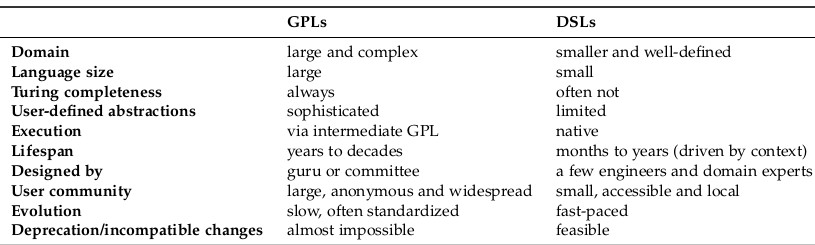
\includegraphics[width=\textwidth]{chapters/fundamentacao/imagens/gplvsdsl.jpg}}

\par\medskip\textbf{Fonte:} \citeonline{dslengineering}. \par\medskip
\end{figure}


Existem situações em que, usuários sem habilidades de programação, precisam injetar regras no sistema, ou definir condições de modo que possam atender uma funcionalidade ou requisito necessário, porém, não é viável ensiná-los conceitos básicos de linguagens de programação. A configuração usando uma linguagem específica de domínio pode ser uma alternativa para resolver estas situações \cite{novak2010easy}.  

No entanto, como em qualquer desenvolvimento de modelagem de software existem benefícios e desafios a serem levados em conta para tomada de decisão sobre adoção \gls{DSL}s no desenvolvimento de software. Na Seção \ref{beneficiosdsl}, são pontuados alguns desses desafios e vantagens encontradas na literatura.

\subsection{Vantagens e desafios no desenvolvimento}
\label{beneficiosdsl}

Para \citeonline{dslengineering}, o uso de \gls{DSL}s no desenvolvimento de soluções traz muitos benefícios, tais como:

\begin{enumerate}
    \item[a)] Produtividade: no sentido de que pode-se substituir muito código fonte de \gls{GPL}s, por algumas poucas linhas de código em \gls{DSL}s;
    
    \item[b)] Qualidade: quando se pensa na criação de um produto com menos \textit{bugs}, resultado da redução do grau de liberdade (desnecessário) para os programadores, prevenindo a duplicação de código (se a \gls{DSL} for projetada da maneira correta);
    
    \item[c)] Validação e Verificação: pois as \gls{DSL}s capturam suas respectivas preocupações de modo que não possuam tantos detalhes de implementação, os programas criados são semanticamente mais ricos que as \gls{GPL}s, permitindo análises e a elaboração de mensagens de erro mais significativas sobre os conceitos do domínio;
    
    \item[d)] Ferramenta de pensamento e comunicação: quando se tem uma maneira de expressar preocupações de domínio, em um idioma que está alinhado com o domínio, o pensamento se torna mais claro, porque o código que você escreve não está cheio de detalhes de implementação. Isso pode estreitar as diferenças de entendimento do domínio, que ocorrem em equipes com várias pessoas trabalhando na solução de um problema em comum;
    
    \item[e)] Envolvimento de especialistas de domínio: quando os especialistas de negócio (não desenvolvedores) conseguem expressar mais facilmente suas ideias, o que pode levar a uma melhor integração entre eles e os desenvolvedores das linguagens;
    
    \item[f)] Ferramentas produtivas: ao contrário de bibliotecas, \textit{frameworks} e \gls{DSL} internas, as \gls{DSL} externas podem ser fornecidas com uma \gls{IDE} preparada para o seu idioma, o que pode resultar em uma experiência de usuário muito aprimorada;

    \item[g)] Redução no \textit{Overhead}: se tratando de \gls{DSL} de geração de código, o gerador pode reduzir abstrações de domínio mais complexas e gerar código mais eficiente, assim como os compiladores das linguagens convencionais otimizam o \textit{bytecode} gerado.
\end{enumerate}

\citeonline{mernik2005and}, \citeonline{ghosh2011dsl} e \citeonline{dslengineering} apresentam em seus textos, alguns desafios e desvantagens que precisam ser consideradas antes da elaboração de uma \gls{DSL}:

\begin{enumerate}
    \item[a)] A modelagem de \gls{DSL} não é trivial, no sentido que exige muita experiência do domínio e expertise em desenvolvimento de linguagens, poucas pessoas possuem ambos;
    \item[b)] Dependendo do tamanho da comunidade de usuários da \gls{DSL}, o desenvolvimento de treinamentos, documentações, suporte e manutenção, pode se tornar um sério problema;
    \item[c)] O custo inicial de desenvolvimento pode ser alto, apesar de poder ser compensado pelo tempo economizado com o aumento da produtividade nos estágios posteriores do ciclo de desenvolvimento;
    \item[d)] A criação descontrolada de linguagens pode resultar em um design inchado, \citeonline{dslengineering} apresenta o termo \textit{DSL Hell}, no qual ao invés de pesquisar por uma \gls{DSL} existente para determinado domínio e aprendê-la, o desenvolvedor acaba por fazer a construção de uma nova linguagem, que pode possivelmente sobrepor implementações já cobertas, mas ainda assim serem incompatíveis entre si;
    \item[e)] A construção de \gls{DSL}s requer mudança no pensamento cultural da organização, pois o método de desenvolvimento é bastante diferente dos métodos tradicionais da engenharia de software, e podem implicar em mudanças significantes em como a equipe de desenvolvedores e usuários trabalham.
    
\end{enumerate}

No sentido de facilitar o design e a criação das linguagens específicas de domínio, atualmente são encontradas várias \gls{IDE}s, algumas delas são listadas na Seção \ref{ferramentasdsl}. Elas têm como objetivo, agregar produtividade para os designers e desenvolvedores, assim como outras vantagens, compensando assim, os eventuais desafios descritos.







\newpage
\subsection{Ferramentas de construção}
\label{ferramentasdsl}

Para \citeonline{voelter2014generic}, as ferramentas desempenham um papel importante no desenvolvimento de software, à medida em que a complexidade do software aumenta, da mesma forma há um aumento na importância em se construir e utilizar ferramentas de apoio.

\citeonline{fowler2005language} apresenta o termo \textit{Language Workbench}, como o ferramental necessário para construir um conjunto de linguagens específicas de domínio. Para ele, essas ferramentas possuem 3 (três) principais definições em comum para criação de \gls{DSL}s:

\begin{enumerate}
    \item[a)] Definem a sintaxe abstrata, que é o modelo da representação abstrata da linguagem;
    \item[b)] Definem um editor, que permita manipulação da representação abstrata;
    \item[c)] Definem um gerador, que descreve como deve ser traduzida a representação abstrata em uma representação executável.
\end{enumerate}

O processo de desenvolvimento de linguagens pode ser facilitado por meio do uso de ferramentas ou de sistemas de criação de linguagens, apesar de existirem vários, todo esse ferramental possui como propósito básico a descrição de linguagens, podendo variar os interpretadores, analisadores, verificadores de consistência e os ambientes de desenvolvimento (\gls{IDE}s) disponibilizadas aos designers \cite{mernik2005and}. 

\begin{citacao}


A maioria dos ambientes de programação são baseados em edição livre de texto, na qual o desenvolvedor manipula o texto de modo a formar palavras e frases. Nesse sentido, é necessário um \textit{parser} para verificar se o texto do programa (sintaxe concreta) possui a sintaxe correta e assim como criar uma \gls{AST} para popular a estrutura de dados a partir da informação extraída da fonte de texto  \cite[p.179,tradução nossa]{dslengineering}.

\end{citacao}


Nos tradicionais compiladores e \gls{IDE}s, os \textit{parsers} precisam ser implementados manualmente, o que requer grande esforço de desenvolvimento. Para uma realidade de construção de uma linguagem tradicional, \gls{GPL}, essa abordagem faz sentido, porém no contexto de \gls{DSL}s as ferramentas permitem gerar um parser a partir de uma gramática, não sendo necessário que o programador crie um \textit{parser} customizado.

\citeonline{dslengineering} categoriza as ferramentas modernas para construção de \gls{DSL}s como \textit{baseadas em parsing} ou ferramentas de \textit{abordagem projecional}. No primeiro caso, a partir da gramática é gerado um \textit{parser}, e no segundo, a \gls{AST} é construída diretamente por ações no editor, na qual é modificada diretamente enquanto o usuário edita o programa (abordagem bem conhecida para editores gráficos em geral, e o padrão \gls{MVC}). 

Para \citeonline{martinfowlerprojectionalediting}, na abordagem de \textit{parsing}, o compilador utiliza o código fonte para gerar uma representação executável do programa, transformando todo o texto em uma representação abstrata que é mantida apenas durante a compilação. (Figura \ref{fig:abordagemparsing}). 

\begin{figure}[h!]
\centering

\caption{\textmd{Abordagem de \textit{parsing}}}
\label{fig:abordagemparsing}
\fcolorbox{gray}{white}{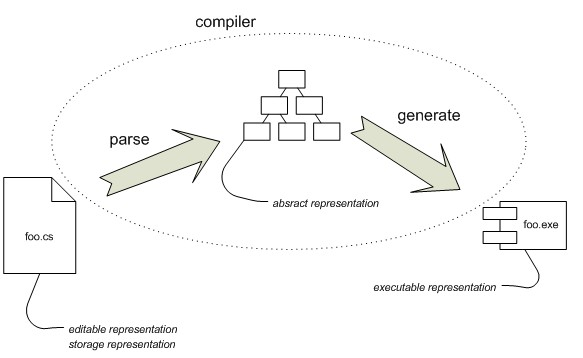
\includegraphics[width=0.8\textwidth]{chapters/fundamentacao/imagens/parsing.jpg}}

\par\medskip\textbf{Fonte:} \citeonline{martinfowlerprojectionalediting}. \par\medskip
\end{figure}


\newpage
No caso da abordagem projecional, utiliza-se editores gráficos para manipular diretamente as definições do sistema, ou seja, edita-se a representação abstrata, de modo que o programador possa modificar as definições mantidas no modelo. Neste caso, o executável é produzido por uma série de projeções e transformações a partir desta representação abstrata (Figura \ref{fig:abordagemprojectional}).


\begin{figure}[ht!]
\centering

\caption{\textmd{Abordagem projecional}}
\label{fig:abordagemprojectional}
\fcolorbox{gray}{white}{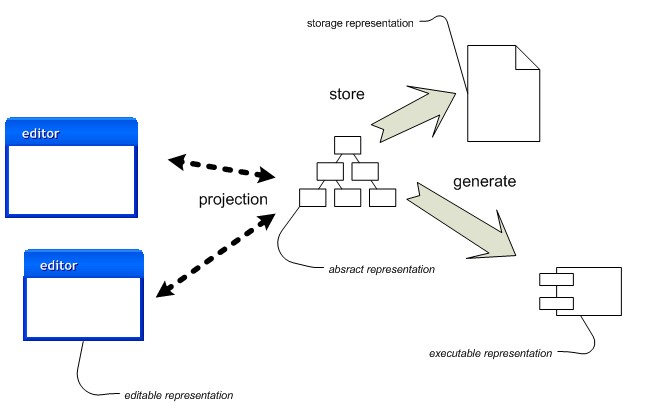
\includegraphics[width=0.8\textwidth]{chapters/fundamentacao/imagens/projectional.jpg}}

\par\medskip\textbf{Fonte:} \cite{martinfowlerprojectionalediting} \par\medskip
\end{figure}

Na Seção \ref{exemplosferramentasdsl} são apresentados alguns exemplos de ferramentas de criação de \gls{DSL}s.

\newpage
\subsection{Exemplos de ferramentas}
\label{exemplosferramentasdsl}

\citeonline{fowler2005language}, apresenta em seu texto, a \textit{Intentional Software} como a precursora das ferramentas de criação de linguagens, foi desenvolvida por \textit{Charles Simonyi} no setor de pesquisa \textit{Microsoft Research}. 

Essa ferramenta permite a criação e edição de código de domínio, o qual é criado por meio da definição de um esquema de domínio pelo \textit{Domain Expert} com apoio dos desenvolvedores, para então ser construído um gerador de código que resulta na aplicação final \cite{simonyi2006intentional}. 

A ferramenta utiliza uma representação de domínio em formato de árvore de intenções, que é apresentada ao usuário em diferentes formas de visualização e edição, a Figura \ref{fig:intentional} mostra a árvore de intenção para uma instrução matemática simples.

\begin{figure}[h!]
\centering

\caption{\textmd{Árvore de intenção no \textit{Intentional Software}}}
\label{fig:intentional}
\fcolorbox{gray}{white}{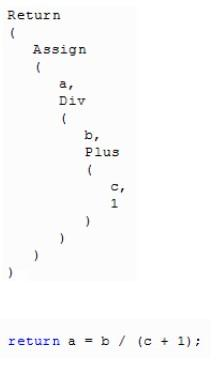
\includegraphics[width=0.4\textwidth]{chapters/fundamentacao/imagens/intentional.jpg}}

\par\medskip\textbf{Fonte:} \cite{simonyi2006intentional} \par\medskip
\end{figure}


Outra ferramenta de abordagem projecional é a \gls{MPS}, de código aberto sob a licença Apache 2.0 e é desenvolvida pela \textit{JetBrains}. Ela se baseia em definição de linguagens por meio de representação de texto estruturado, e possui uma série de recursos sofisticados de edição e ferramentas de navegação. 

Segundo \citeonline{dslengineering}, a \gls{MPS} suporta notações mistas (textuais, simbólicas, tabulares, gráficas) e uma ampla variedade de recursos de composição de idiomas. Ela define a linguagem por meio de \textit{Concepts} que são elementos para criação da sintaxe abstrata (Figura \ref{fig:mpsconceitos}), e esses conceitos são atrelados a um editor, o qual define as regras de projeção por meio de uma lista de células, que juntas definem a estrutura desejada para a sintaxe do conceito (Figura \ref{fig:mpseditor}).

\begin{figure}[h!]
\centering

\caption{\textmd{MPS definição de Conceitos}}
\label{fig:mpsconceitos}
\fcolorbox{gray}{white}{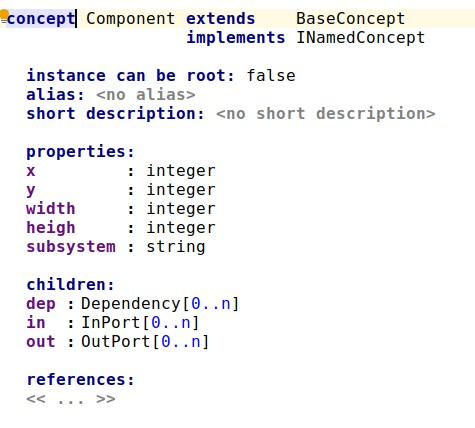
\includegraphics[width=\textwidth]{chapters/fundamentacao/imagens/mpsconceitos.jpg}}

\par\medskip\textbf{Fonte:} JetBrains (2018). \par\medskip
\end{figure}


\begin{figure}[ht!]
\centering

\caption{\textmd{MPS editor - sintaxe abstrata}}
\label{fig:mpseditor}
\fcolorbox{gray}{white}{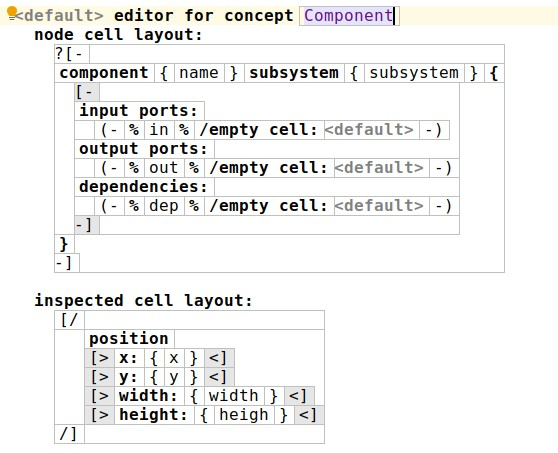
\includegraphics[width=0.98\textwidth]{chapters/fundamentacao/imagens/mpseditor.jpg}}

\par\medskip\textbf{Fonte:} JetBrains (2018). \par\medskip
\end{figure}


\newpage


Como alternativa às ferramentas projecionais, existem ferramentas que geram o \textit{parser} a partir da gramática, nesse caso, as regras da linguagem são expressadas em notação baseada em \gls{BNF}. As ferramentas Xtext e Spoofax são casos de ambientes nos quais é possível construir \gls{DSL}s por meio desse tipo de abordagem, a seguir são listados alguns exemplos nessas ferramentas.


\citeonline{eysholdt2010xtext}, descreve a ferramenta Xtext, como um \textit{framework} que permite o rápido desenvolvimento de ferramental de suporte às linguagens textuais, podendo atender desde linguagens menores como \gls{DSL}s, até linguagens completas \gls{GPL}s. Ela utiliza o core do \gls{EMF} para criar a \GLS{AST} a partir de uma especificação de gramática. 

Na Figura \ref{fig:xtextgramatica} é possível verificar a definição da gramática de uma linguagem específica para modelagem de entidades, de forma similar ao que existe em alguns \textit{frameworks} de programação, como Rails e Grails. O resultado é apresentado na Figura \ref{fig:xtextprograma}, na qual observa-se a utilização de recursos do Xtext no momento da codificação de um novo programa nessa linguagem.

\begin{figure}[ht!]
\centering

\caption{\textmd{Exemplo de definição de gramática Xtext}}
\label{fig:xtextgramatica}
\fcolorbox{gray}{white}{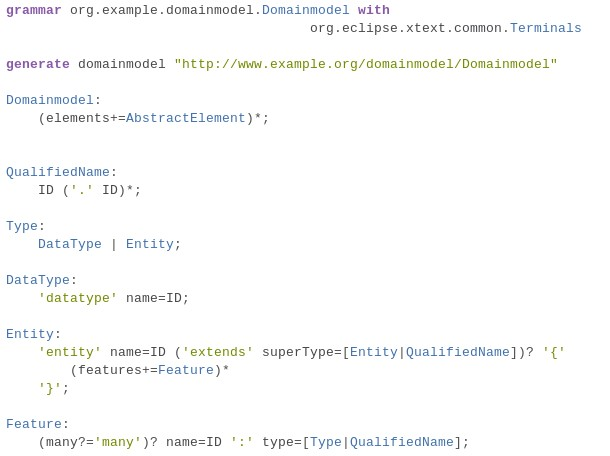
\includegraphics[width=0.9\textwidth]{chapters/fundamentacao/imagens/xtextgramatica.jpg}}

\par\medskip\textbf{Fonte:} \citeonline{xtextsite}. \par\medskip
\end{figure}


\begin{figure}[h!]
\centering

\caption{\textmd{Exemplo de uso da linguagem de entidades}}
\label{fig:xtextprograma}
\fcolorbox{gray}{white}{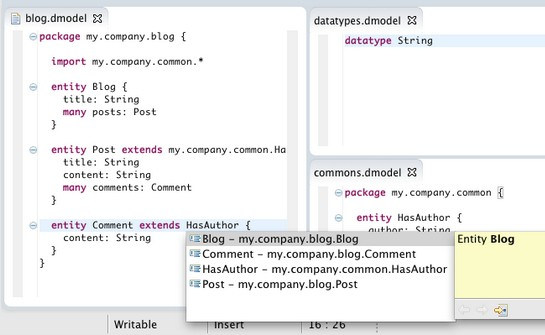
\includegraphics[width=0.9\textwidth]{chapters/fundamentacao/imagens/xtextprograma.jpg}}

\par\medskip\textbf{Fonte:} \citeonline{xtextsite}. \par\medskip
\end{figure}


\newpage
Por fim, a ferramenta \textit{Spoofax} utiliza o formato \gls{SDF} para descrição da sintaxe da linguagem, sendo um ambiente integrado de especificação de linguagens, com suporte e \textit{plugins} para a \gls{IDE} Eclipse. 

Um exemplo de definição de gramática em formato \gls{SDF} pode ser observado na Figura \ref{fig:spoofaxgramatica}. No canto esquerdo da imagem são definidas as regras da sintaxe, para uma linguagem de entidades similar a que foi utilizada no exemplo do Xtext. 

\begin{figure}[h!]
\centering

\caption{\textmd{Definição de gramática no Spoofax}}
\label{fig:spoofaxgramatica}
\fcolorbox{gray}{white}{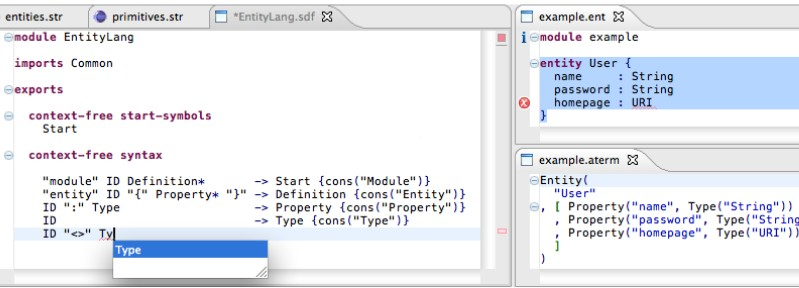
\includegraphics[width=0.9\textwidth]{chapters/fundamentacao/imagens/spoofaxgramatica.jpg}}

\par\medskip\textbf{Fonte:} \cite{kats2010spoofax} \par\medskip
\end{figure}



Segundo \citeonline{kats2010spoofax}, os seus editores permitem verificar e destacar erros por linha, validar tipos de dados da linguagem, resolução de referências, recursos de ajuda conforme contexto e até completar ou sugerir opções de código para o usuário da linguagem (Figura \ref{fig:spoofaxeditor}). 

\begin{figure}[h!]
\centering

\caption{\textmd{Recursos do editor Spoofax}}
\label{fig:spoofaxeditor}
\fcolorbox{gray}{white}{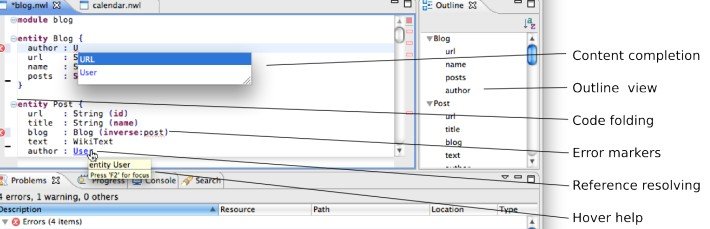
\includegraphics[width=\textwidth]{chapters/fundamentacao/imagens/spoofaxeditor.jpg}}

\par\medskip\textbf{Fonte:} \cite{kats2010spoofax} \par\medskip
\end{figure}


A fim de criar a linguagem de domínio proposta pelo presente trabalho, será necessário definir entre uma dessas ferramentas. Na Seção \ref{justificativamps} é apresentada a justificativa da escolha do \gls{MPS} como ferramenta para implementação da linguagem de especificação de regras de classificação pelo sistema de cotas.

\subsection{Justificativa de escolha da ferramenta MPS}
\label{justificativamps}


%artigo marting fowler , defining a language workbench
